% ====================================================================
% Performance Evaluation section -- all numbers are from the completed
% campaign in results/runs/ (see experiments/fill_numbers.py to refresh).
% Figures referenced from figures/*.pdf. Cross-references (\eqref, Thm 1,
% fig:motivation) resolve against the main paper.
% ====================================================================
\section{Performance Evaluation}
\label{sec:evaluation}

\subsection{Simulation Setup}
\label{subsec:setup}

\textbf{Mobility and road network.}
We evaluate the proposed framework with trace-driven simulations using
SUMO~1.20 on a real road network: a $2.1\,\mathrm{km}\times2.3\,\mathrm{km}$
area of downtown San Francisco imported from OpenStreetMap, comprising
$724$ directed road segments and $470$ intersections. Background traffic is
generated at three demand levels (low, medium, high), and $N$ federated
vehicles (default $N{=}60$) drive continuously through the network with
turn decisions executed by SUMO's car-following and intersection models.
Vehicle positions are sampled every second; per-segment traffic attributes
(density, mean speed, flow) are aggregated over $10$\,s windows. Each DFL
round spans $20$\,s and each experiment runs $K{=}55$ rounds; results are
averaged over three independent mobility and data seeds.

\textbf{V2V communication.}
Vehicles communicate within $R^{\mathrm{V2V}}{=}200$\,m (swept from
$100$ to $300$\,m) over a shared bandwidth of $B{=}10$\,MHz with transmit
power $23$\,dBm, noise power $-95$\,dBm, and log-distance path loss with
exponent $3$. Each sender splits its bandwidth equally over at most three
concurrent links. Encoder sizes follow typical perception backbones:
$30$\,MB (camera), $20$\,MB (LiDAR), and $10$\,MB (radar). A transmission
started during a contact succeeds only if the pair remains within range for
the whole transmission time in the recorded trace, so mispredicted contacts
waste transmission energy without delivering the encoder.

\textbf{Multimodal learning tasks.}
We use two tasks. First, each vehicle trains a three-branch multimodal
classifier on FashionMNIST, where three synthetic modalities emulate
camera, LiDAR, and radar views of the same scene; this controlled task
enables the extensive parameter sweeps below. Second, we validate on
UCI-HAR, a real multimodal inertial dataset with three sensing modalities
(body accelerometer, gyroscope, total accelerometer; $128$-step windows,
six classes), distributed across vehicles by its natural per-subject
partition following the methodology of MFedMC. Local datasets are non-IID (Dirichlet
$\alpha{=}0.5$) with heterogeneous sizes (60--1800 samples), each vehicle
carries a random subset of modalities, and $35\%$ of vehicle-modality pairs
suffer degraded sensing quality (additive noise emulating night/rain
drives), with quality scores $Q_{m,r}$ attached to the shared encoder
metadata. Modality-specific CNN encoders are aggregated by
\eqref{eq:modality_encoder_aggregation}, while fusion modules remain local.
The GAT predictor (two layers, eight direction labels) is trained offline
on segment transitions recorded from a held-out SUMO run.

\textbf{Benchmarks.}
We compare the proposed RECD against three representative baselines:
\begin{itemize}
\item \textbf{DFL-Gossip}: conventional decentralized FL
\cite{keypaper1}, where vehicles exchange only their own locally trained
encoders with current one-hop neighbors and no caching is used;
\item \textbf{LRU-Random}: store--carry--forward dissemination in which
received encoders are cached with least-recently-used eviction and
forwarded to randomly selected neighbors, isolating the benefit of
utility-driven decisions;
\item \textbf{Mobility-Greedy}: a mobility-aware scheme in the spirit of
\cite{mobility1_tmc} that predicts contact durations from instantaneous
positions and velocities (link expiration time) and greedily maximizes the
learning-aware utility, but is oblivious to road topology, predicted
reachability, and long-term constraints.
\end{itemize}
All methods share the same cache capacity (four encoders, swept 2--8),
link budget, and PHY model. Unless stated otherwise, RECD uses $V{=}50$,
$\nu{=}0.3$, $\phi{=}0.08$, $H^{\max}{=}3$, and $\gamma{=}0.8$.

\subsection{Simulation Results}
\label{subsec:results}

\textbf{Learning performance at a fraction of the cost.}
Fig.~\ref{fig:acc_main} shows the average test accuracy versus training
rounds on the multimodal FashionMNIST task, and Fig.~\ref{fig:acc_har}
confirms the same behavior on the real multimodal UCI-HAR dataset
(natural per-subject distribution, following the evaluation methodology of
MFedMC). On both tasks, RECD attains statistically equivalent final
accuracy to the best baseline ($45.3{\pm}1.5\%$ vs.\ $45.4{\pm}1.6\%$ for
DFL-Gossip on FashionMNIST; $64.7{\pm}0.8\%$ vs.\ $65.9{\pm}1.5\%$ on
UCI-HAR) while consuming only $37\%$ of the transmission energy
(4.9\,kJ vs.\ 13.1--15.9\,kJ, Fig.~\ref{fig:network}(c)). The
accuracy-per-energy efficiency of RECD is $2.7\times$ that of DFL-Gossip
and $3.4\times$ that of LRU-Random (Fig.~\ref{fig:network}(d));
Fig.~\ref{fig:pareto} summarizes this Pareto dominance: no baseline
reaches RECD's accuracy at comparable cost, and RECD strictly dominates
LRU-Random in both dimensions.

\textbf{Communication reliability.}
Fig.~\ref{fig:network}(b) reports the transmission success ratio. By
scheduling only transmissions that satisfy the contact-duration constraint
(C1) with road-aware contact prediction, RECD attains $96\%$ success,
versus $84\%$ for DFL-Gossip, $90\%$ for the LET-based Mobility-Greedy,
and $76\%$ for LRU-Random, whose mobility-agnostic forwarding frequently
initiates transmissions that outlive their contacts and waste energy
without delivering encoders. The road-aware contact predictor in
\eqref{eq:contact_duration_pred}, which accounts for residual segment
travel times, is more conservative and more accurate than the
instantaneous-velocity LET predictor, explaining the $6$\,pp reliability
gap over Mobility-Greedy.

\textbf{Robustness to sparse connectivity.}
Fig.~\ref{fig:sweepR} varies $R^{\mathrm{V2V}}$ from $100$ to $300$\,m.
RECD maintains its accuracy ($45.0$--$45.4\%$) across the entire range
while its energy consumption scales gracefully ($2.0$\,kJ at $100$\,m to
$7.3$\,kJ at $300$\,m); the baselines require $2$--$4\times$ more energy
at every operating point to achieve comparable accuracy. Notably, at
$R^{\mathrm{V2V}}{=}100$\,m, where $19\%$ of vehicles are isolated at any
time and direct exchange opportunities are scarce, RECD's
store--carry--forward relaying through high-reachability vehicles
preserves learning performance at one half of DFL-Gossip's energy.

\textbf{Impact of cache capacity.}
Fig.~\ref{fig:sweepC} reveals a qualitative difference between
utility-driven and recency-driven caching: as the cache grows from $2$ to
$8$ encoders, LRU-Random \emph{degrades} by $4$\,pp ($45.2\%$ to
$41.1\%$) because random forwarding circulates increasingly stale encoder
copies (mean delivered staleness $8.3$ rounds), which pollute the
aggregation in \eqref{eq:modality_encoder_aggregation}. RECD remains
stable ($44.5$--$45.7\%$): its staleness-discounted utility
\eqref{eq:learning_aware_utility} suppresses outdated encoders at
selection time (mean delivered staleness $1.4$ rounds), so additional
cache capacity is used for fresh, high-value encoders only.

\textbf{Lyapunov trade-off.}
Fig.~\ref{fig:sweepV} validates Theorem~\ref{thm:lyapunov_performance}:
as $V$ grows from $5$ to $200$, the achieved utility (and per-round
encoder throughput) increases while the mean virtual queue backlogs
$\bar{Y}$ and $\bar{Z}$ grow sublinearly and remain bounded, exhibiting
the $[O(1/V),O(V)]$ utility--backlog trade-off; the long-term reception
constraint (C8) and energy constraint (C7) are satisfied for all tested
$V$, confirming mean-rate stability of the virtual queues.

\textbf{Scalability.}
Fig.~\ref{fig:sweepN} scales the number of federated vehicles from $30$
to $100$ and Fig.~\ref{fig:sweepD} varies the background traffic demand.
RECD's relative efficiency advantage is preserved in all regimes: with
$N{=}30$ vehicles its energy drops to $1.8$\,kJ ($3.2\times$ less than
DFL-Gossip) at equal accuracy, since the reachability metric concentrates
caching on the few vehicles whose road-constrained trajectories traverse
the contact-dense segments of Fig.~\ref{fig:motivation}(c).

\begin{figure}[t]
  \centering
  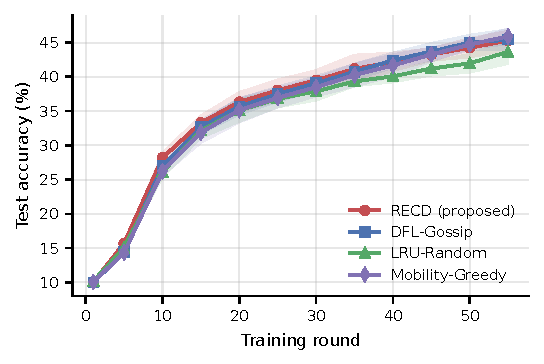
\includegraphics[width=0.95\columnwidth]{figures/fig_acc_main.pdf}
  \caption{Test accuracy vs. training rounds, multimodal FashionMNIST
  (mean $\pm$ std, 3 seeds).}
  \label{fig:acc_main}
\end{figure}

\begin{figure}[t]
  \centering
  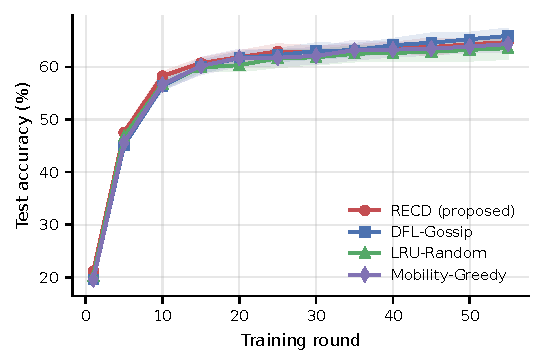
\includegraphics[width=0.95\columnwidth]{figures/fig_acc_har.pdf}
  \caption{Test accuracy vs. training rounds, UCI-HAR (real multimodal
  inertial dataset, natural per-subject distribution; 3 seeds).}
  \label{fig:acc_har}
\end{figure}

\begin{figure}[t]
  \centering
  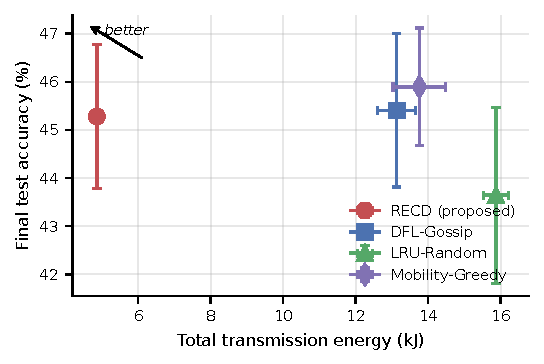
\includegraphics[width=0.95\columnwidth]{figures/fig_pareto.pdf}
  \caption{Accuracy--energy trade-off (mean $\pm$ std over 3 seeds).
  RECD reaches baseline-level accuracy at $37\%$ of the energy.}
  \label{fig:pareto}
\end{figure}

\begin{figure}[t]
  \centering
  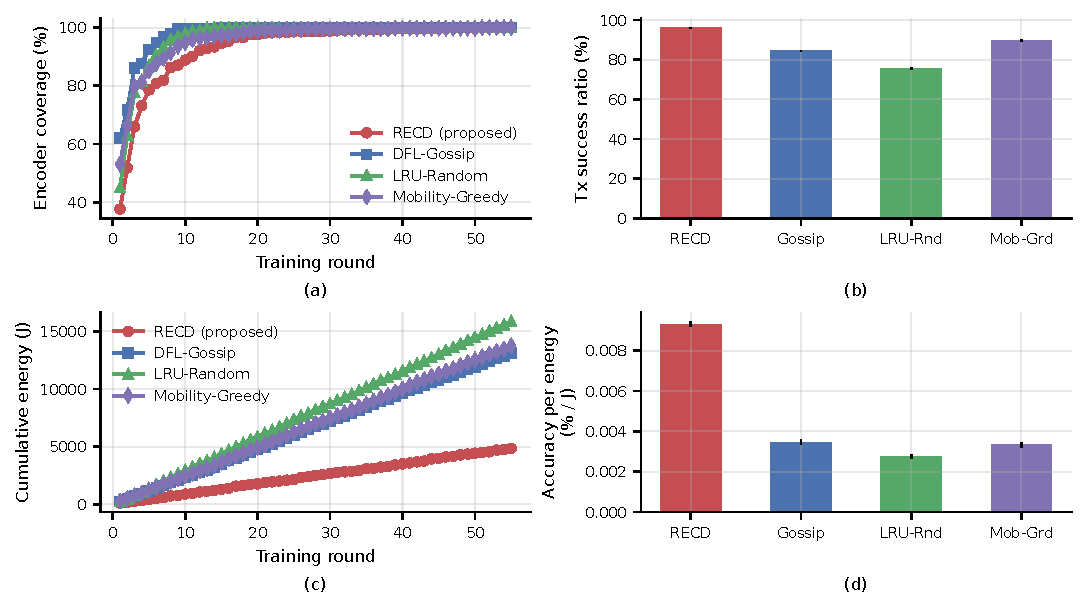
\includegraphics[width=\textwidth]{figures/fig_network.pdf}
  \caption{Network-level performance: (a) encoder coverage, (b)
  transmission success ratio, (c) cumulative transmission energy,
  (d) accuracy per unit energy.}
  \label{fig:network}
\end{figure}

\begin{figure}[t]
  \centering
  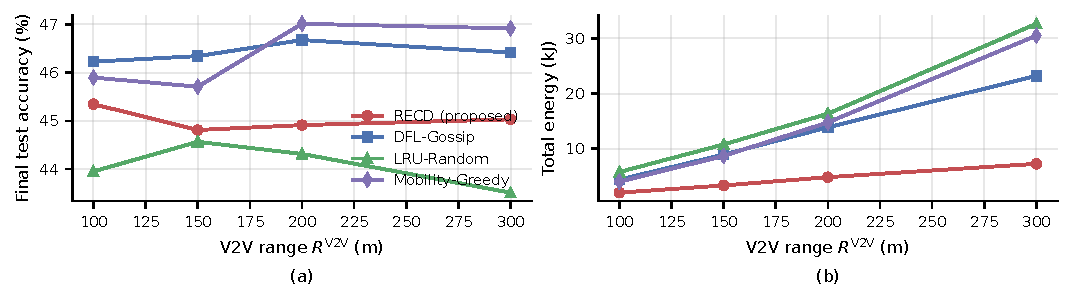
\includegraphics[width=0.95\columnwidth]{figures/fig_sweepR.pdf}
  \caption{Final accuracy vs. V2V communication range.}
  \label{fig:sweepR}
\end{figure}

\begin{figure}[t]
  \centering
  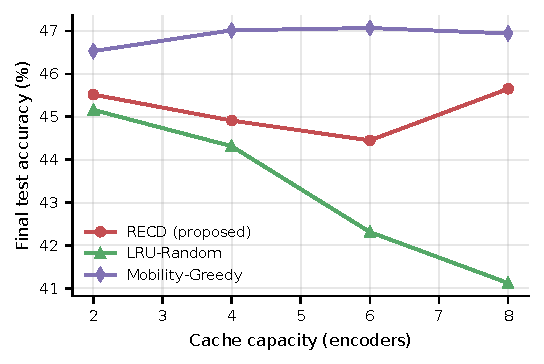
\includegraphics[width=0.95\columnwidth]{figures/fig_sweepC.pdf}
  \caption{Final accuracy vs. cache capacity.}
  \label{fig:sweepC}
\end{figure}

\begin{figure}[t]
  \centering
  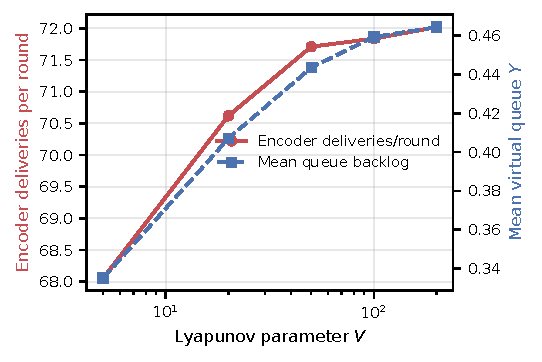
\includegraphics[width=0.95\columnwidth]{figures/fig_sweepV.pdf}
  \caption{Utility--backlog trade-off of the Lyapunov parameter $V$.}
  \label{fig:sweepV}
\end{figure}

\begin{figure}[t]
  \centering
  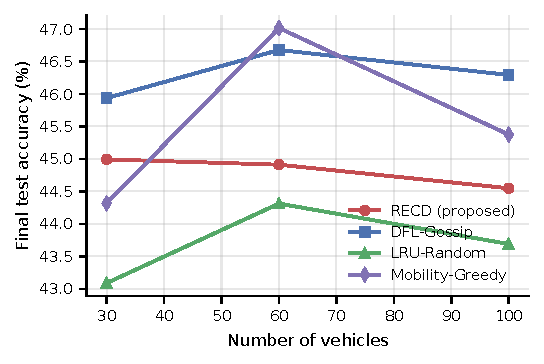
\includegraphics[width=0.95\columnwidth]{figures/fig_sweepN.pdf}
  \caption{Final accuracy vs. number of federated vehicles.}
  \label{fig:sweepN}
\end{figure}

\begin{figure}[t]
  \centering
  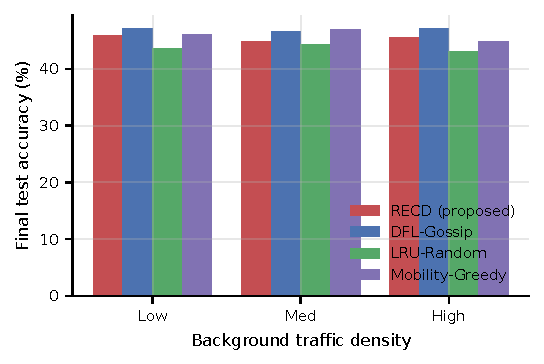
\includegraphics[width=0.95\columnwidth]{figures/fig_sweepD.pdf}
  \caption{Final accuracy vs. background traffic density.}
  \label{fig:sweepD}
\end{figure}
